\documentclass{article}
\usepackage{graphicx}

\usepackage[english]{babel}

\begin{document}

cloud data
 \begin{table}
 \small
 \begin{tabular}{|c|c|c|c|c|c|c|} 
 \hline 
 Case&Read File&Threads  & \# of & Total & \# of  &  $T_C$  \\ 
     & Size (MB) & per Task & Tasks & Cores &  VM's & seconds \\ 
\hline
c1 & 800  &8 & 1 &  8 & 1 &2001  \\\hline
c2 & 400 &4 & 2 &  8 & 1 &921 \\\hline
c3 & 200 &2 & 4 &  8 & 1 &569 \\\hline
c4 & 100 &1 & 8 &  8 & 1 &366 \\\hline

\hline

 \end{tabular}

 \caption{ The number of index files used for this measurement is 10(1.7 GB).
   In all cases the input and output data resides on VM itself.  VM in
   case c1 c2, c3, c4 are of type c1.xlarge }
  \label{table:cloud-VM} 
\end{table}



\begin{table}
\scriptsize
 \begin{tabular}{|c|c|c|c|c|c|c|c|} 
 \hline 
Case &Genome & Index         & Resource    & \# of & \# of &   \# of         &	TTC  \\
  &Type               & File (GB)        & &Cores &   nodes &  Tasks&  (sec)\\  
\hline
FG1 &Chr &1.7& India	&	8& 1 & 8&605 \\
\hline
FG2 &Chr &1.7& India	&	16&2&16	&  717 \\
\hline
FG3 &Chr &1.7& India	&	24&3&24	&  851 \\
\hline
FG4 &Chr &1.7& Cyder &	8 & 1&8	& 766 \\
\hline
FG5 &Chr &1.7& India/Cyder &	8/8& 1/1& 16 & 783 \\
\hline
FG6 &Chr &1.7& India/Cyder &	16/8& 2/1& 24 & 772 \\
\hline

\end{tabular}
\caption{
In this tables just number of tasks are varied but all tasks have the same read file size ie total amount of  read files data processed is varied with number of tasks.
Cyder (12 core local workstation).
India (FG machine).
all tasks  read file size 136MB.
FG3 VS FG6 clearly shows the I/O boundedness of number of tasks.
FG5 VS FG6 clearly there is unpredictable minor coordination cost involved.
But this minor difference will get bigger and bigger with entire Human genome and/or when single read file  size is increased
}

  \label{table:NGS-Distributed} 
\end{table}









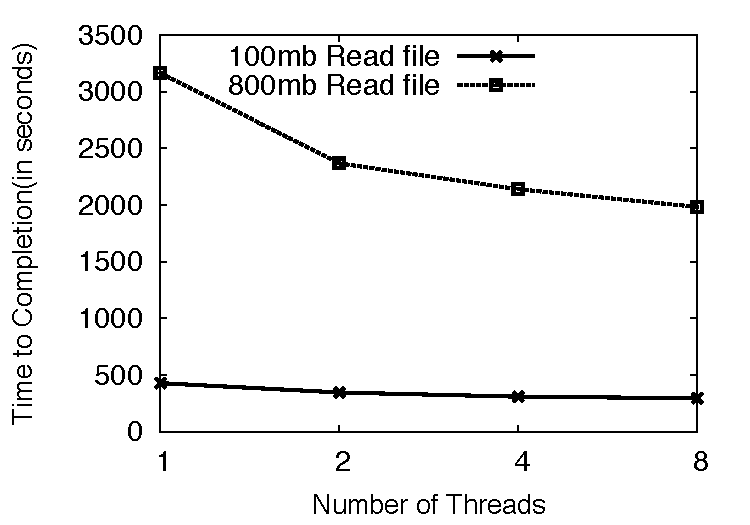
\includegraphics[scale=0.66]{../figures/cloud_threadsvstime.pdf} 



\end{document}

